\documentclass[osajnl,twocolumn,showpacs,superscriptaddress,10pt]{revtex4-2}
%
\usepackage{dcolumn}% Align table columns on decimal point
\usepackage{bm}% bold math
%
%Paquete de Idioma
\usepackage[spanish]{babel}
%
%Codificación Alfabeto
\usepackage[utf8]{inputenc}
%
%Codificación de Fuente
\usepackage[T1]{fontenc}
%
%Índice
\usepackage{makeidx}
%
%Gráficos
\usepackage{graphicx}
\usepackage{subfig}
%
%Matemática
\usepackage{amsmath}
\usepackage{amsfonts}
\usepackage{amssymb}




%\usepackage{amstext} 
%
%Estilo de Página Numeración superior
%\pagestyle{headings}
%
%Hiperlinks \href{url}{text}
\usepackage[pdftex]{hyperref}
%
%Graficos y tablas
\usepackage{multirow}
%\usepackage{multicol}
\usepackage{float}
\usepackage{booktabs}
\usepackage{cancel}
%\usepackage{tikz-feynman}

\usepackage[table,xcdraw]{xcolor}
\usepackage[utf8]{inputenc}
\usepackage{tikz}
\usetikzlibrary{shapes,snakes}
\usetikzlibrary{arrows.meta}
\usetikzlibrary{calc,patterns,angles,quotes}
\usepackage{siunitx}
%\tikzfeynmanset{compat=1.0.0}
%

%
%
\begin{document}
	%Titulo
	\title{La paradoja EPR y la desigualdad de Bell}
	
	\author{Rubí Esmeralda, Ramírez Milián, 201804565$^1$ y Jorge Alejandro, Rodríguez Aldana, 201804766}
	\affiliation{ECFM, Departamento de Física, Universidad de San Carlos, Edificio T1, Ciudad Universitaria, Zona 12, Guatemala.
	}
	
	
	%\collaboration{MUSO Collaboration}%\noaffiliation
	
	%\date{\today}%
	
	%Resumen
	\begin{abstract}
		
		
	\end{abstract}
	
	\maketitle{}
	
	\section{Introducci\'on }
	
	
	

	\section{Métrica Minkowski}
	
	El espacio-tiempo de Minkowski es un conjunto de cuatro dimensiones, con elementos etiquetados por tres dimensiones espaciales y una temporal. Un punto individual en el espacio tiempo es llamado un evento. La trayectoria de una partícula es una curva a través del espacio-tiempo. 
	
	
	
	EL intervalo entre dos eventos en el espacio tiempo está descrito:
	$$(\Delta s)^2=-(c\Delta t)^2+(\Delta x)^{2}+(\Delta y)^{2}+(\Delta z)^{2}$$
	
	
	
	
	donde $c$ es la velocidad de la luz en el vacío. Lo inportante en está definición de intervalo del espacio-tiempo entre dos eventos es que es \textit{invariante bajo trnasformaciones de coordenadas inerciales}. No existe una noción absoluta de "eventos simultáneos"; es decir si dos cosas ocurren al mismo tiempo depende de las coordenadas utilizadas.

	El espacio-tiempo tiene un tensor métrico asociado que puede escribirse en forma matricial como
$${\displaystyle \left(\eta _{\alpha \beta }\right):={\begin{pmatrix}-1&0&0&0\\0&1&0&0\\0&0&1&0\\0&0&0&1\end{pmatrix}}} $$
	
%{\overset {\underset {\mathrm {def} }{}}{=}}
Ahora el intervalo del espacio tiempo entre dos eventos escrito en forma tensorial:


	$$(\Delta s)^{2}= -\eta_{\mu \nu }\Delta x^{\mu}\Delta x^{\nu}$$
	

Una herramienta muy útil para comprender el espacio-tiempo es la estructura del cono de luz que están dividos en futuro y pasado. Todos los punto dentro del cono de luz futuro y pasado de  un evento <<O>> en el espacio tiempo, son llamados puntos \textit{timelike} con $(\Delta s)^{2} > 0 $. Y  los puntos de los conos son \textit{light-like} o nulos $ (\Delta s)^{2}=0 $ .Si se supone que todos los procesos causales se propagan a la velocidad de la luz o a una velocidad menor, se concluye que estos son todos los eventos que se pueden afectar causalmente a partir de O. 
%El cono de luz futuro en O contiene todos los eventos en el espacio-tiempo a los que se puede llegar desde O mediante curvas de luz o de tiempo dirigidas por el futuro. 

Los puntos que  están fuera del cono de luz del evento O están separado en forma \textit{space-like} con $ (\Delta s)^{2}<0 $.  Si se asume que ningún proceso causal se propaga más rápido que la luz, estos eventos están causalmente desconectados de O. 



%\input{EPR-Bell.tex}


	

	

	
	\section{Paradoja de EPR}

% Partamos, suponiendo que la mecánica cuántica es una teoría local, de modo que 

Si tenemos dos partículas entrelazadas, sabemos que al medir una de ellas, se definirá en un estado, y por tanto, la otra también lo hará. El problema con esto, es que, aparentemente, tenemos dos eventos directamente relacionados, ocurriendo al mismo tiempo, lo que parece una contradicción a la Relatividad.

% Veamos cual es el error de este planteamiento; para que la mecánica cuántica siga las reglas de la Relatividad, debe ser una teoría local, y por tanto

% \input{Geogebra/EPR-Bell.tex}

\begin{figure}[H]
    \centering
    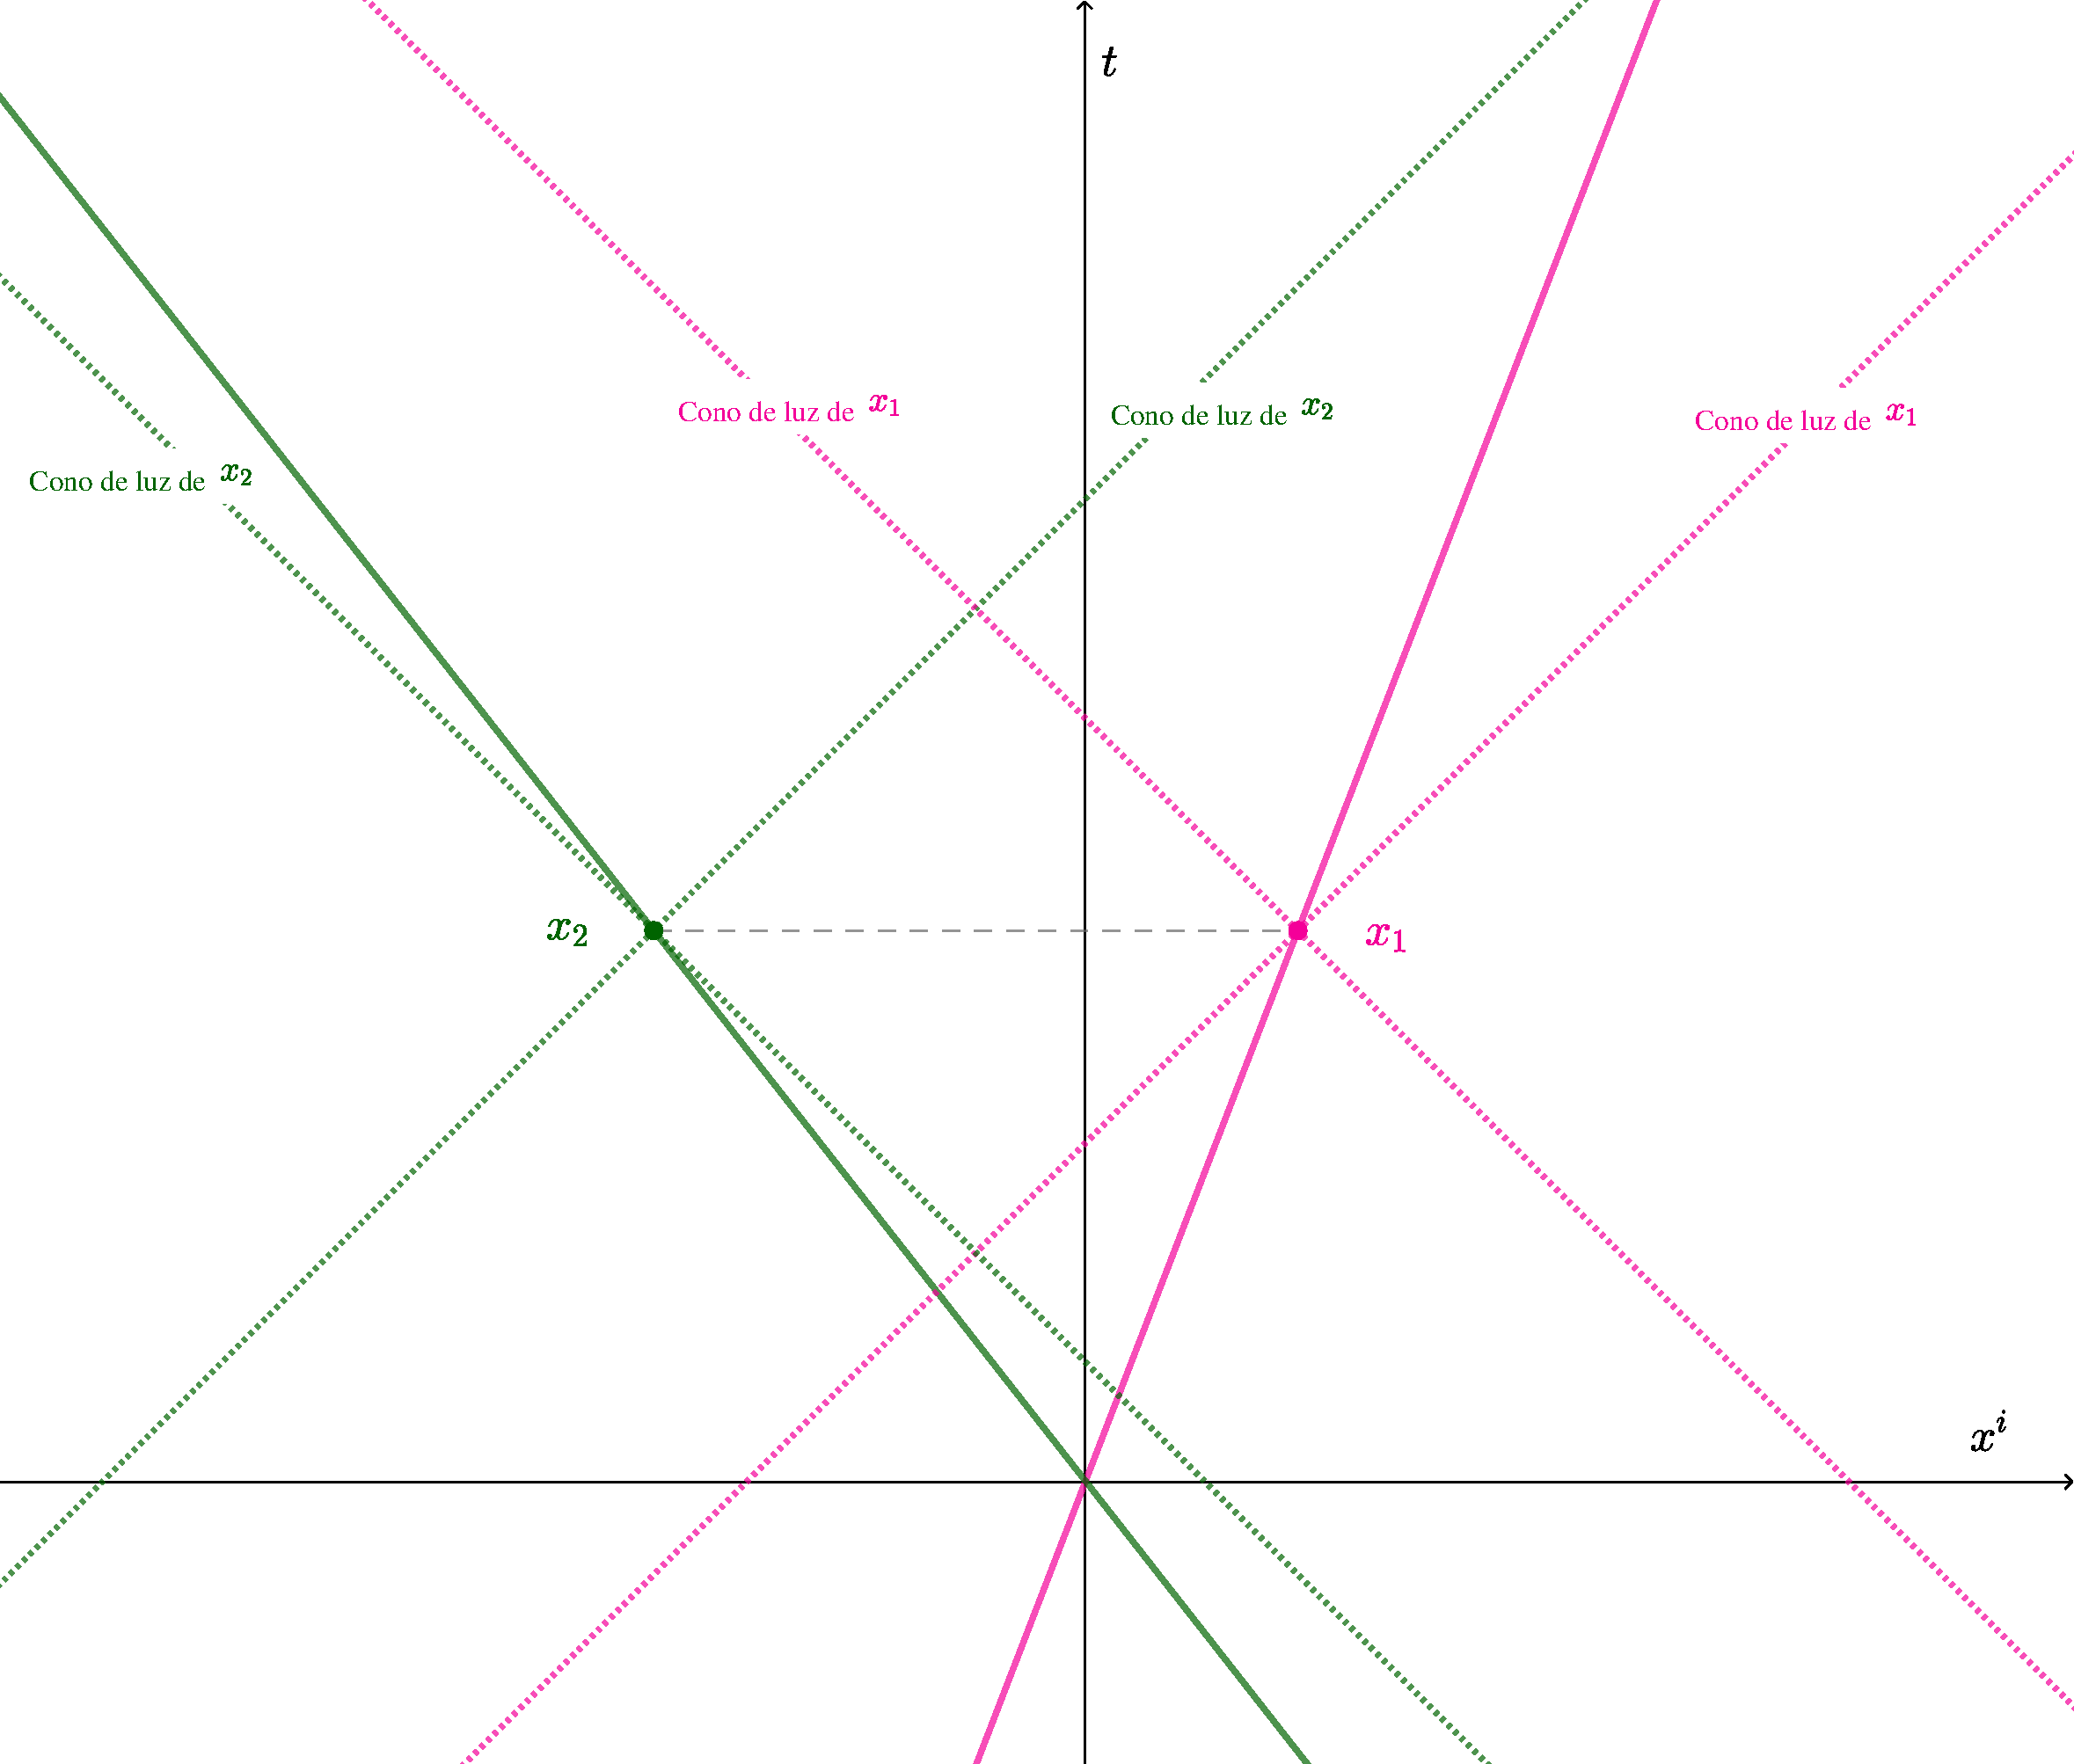
\includegraphics[width=0.4\textwidth]{Graphics/SpaceLike.pdf}
    \label{fig:SpaceLike}
    \caption{Diagrama de Minkowski}
\end{figure}
\bigskip

Veamos este planteamiento con más rigurosidad matemática:

\medskip

Sean $\mathbf{x_1}$ y $\mathbf{x_2}$, dos partículas observadas por un mismo observador en un sistema inercial, que se entrelazan en $t=0$ y luego se alejan a velocidades $\mathbf{v_1}$ y $\mathbf{v_2}$ respectivamente. Entonces tenemos:

\begin{align*}
    \mathbf{x_1} &= \left(x^0_1,x^1_1,x^2_1,x^3_1\right)\\
    \mathbf{x_2} &= \left(x^0_2,x^1_2,x^2_2,x^3_2\right)
\end{align*}

Pero, al ser observados por un mismo observador, partiendo de un mismo evento, entonces: $x^0_1=x^0_2=t$:

\begin{align*}
    \mathbf{x_1} &= \left(t,x^1_1,x^2_1,x^3_1\right)\\
    \mathbf{x_2} &= \left(t,x^1_2,x^2_2,x^3_2\right)
\end{align*}

Y suponiendo una velocidad constante, entonces $x^i_n=tv^i_n$:

\begin{align}
    \mathbf{x_1} &= \left(t,tv^1_1,tv^2_1,tv^3_1\right)\\
    \mathbf{x_2} &= \left(t,tv^1_2,tv^2_2,tv^3_2\right)
\end{align}

Calculemos entonces $\Delta x^\alpha$

\begin{align*}
    \Delta x^\alpha 
        &:= \left(x^\alpha_2-x^\alpha_1\right)\\
    \Delta x^0
        &= \left(t-t\right)=0\\
    \Delta x^i
        &= \left(x^i_2-x^i_1\right)\\
        &= \left(tv^i_2-tv^i_1\right)\\
        &= t\left(v^i_2-v^i_1\right)\\
        &= t\Delta v^i
\end{align*}

Calculemos ahora $\Delta s^2$

\begin{align*}
    \Delta s^2 
        &:= -\eta_{\alpha\beta}\Delta x^\alpha \Delta x^\beta\\
        &=-\eta_{00}~\cancelto{0}{\left(\Delta x^0\right)^2}-\cancelto{\delta_{ij}}{\eta_{ij}}~~~~~\left(\Delta x^i\Delta x^j\right)\\
        &=0-\delta_{ij}\left(\Delta x^i\Delta x^j \right)\\
        &=\sum_{i=1}^3-\left(\Delta x^i\right)^2\\
        &=-t^2\sum_{i=1}^3 \left(\Delta v^i\right)^2\\
        &=-t^2\left[\left(\Delta v^1\right)^2+\left(\Delta v^2\right)^2+\left(\Delta v^3\right)^2\right]\\
        &\leq0
\end{align*}

El caso de la igualdad solo se da en $t=0$ o si las velocidades de ambas partículas son las mismas, de modo que $\Delta v^i = 0~~\forall~i\in[1,3]$

Y por tanto, en el caso que las velocidades sean distintas, la métrica de Minkowski es menor a cero, es decir, los eventos $x_1$ y $x_2$ no tienen una relación causal. Y al estar correlacionados, esto es una aparente violación de la teoría de la Relatividad.


	
	%\input{EPR-Bell.tex}
	
	
	
	
	
	
	
	
	\section{Conclusi\'on}
	
	
	
	\nocite*
	\bibliographystyle{IEEEtran}
	\bibliography{IEEEabrv,referencias}
	
\end{document}
